\chapter{Background}

This chapter introduces the concepts which form the building blocks for our
iptables model, making use of the extensive work conducted by Stoenescu et. al
\cite{stoenescu2013symnet, stoenescu2016symnet}.

We first give a short overview of the broad field of network verification, with
an emphasis on the approach that we use: static verification powered by
symbolic execution.  We then show how it is implemented in SymNet, and how
SymNet can be used to verify the models we build.  Finally, we go into details
about iptables; we discuss its internal organization, as well as its most
common features.

\section{Network verification}\label{sec:network-verification}
\todo{what is \emph{formal verification}}

\paragraph{Correctness.}\label{par:correctness}
Network verification is merely formal verification tailored for network-related
questions.  But in order to do so, we need to provide a rigorous definition for
network correctness.  It turns out that this is by itself a very involved task.
Being abstract is what one might try in order to get around this formalism:

\begin{definition}[Network correctness]
\label{def:full-correctness}
A network behaves correctly as long as it complies to operator's policy.
\end{definition}

At first, this definition does not seem to accomplish much, as what it
essentially does is to delegate the requirement by introducing the need to
formally define a \emph{policy}, or, more precisely, its composing rules.
Therefore, the follow-up question that arises is:

\begin{quote}
What is a (policy) rule and how is it specified?
\end{quote}

In fact, there is ongoing work that focuses on bringing policy specification
closer to the natural language, on one hand, and the automation of policy
proving, on the other hand.  The latter, called \textbf{policy-driven network
verification}, could significantly reduce verification run-times, similar to
the way \emph{informed search} algorithms compare to the uninformed ones on
large search spaces.  Another analogy stems from the field of automatic theorem
proving: policy-based verification resembles the \emph{forward chaining}
inference method, by propagating packets through the modelled network (a
procedure further detailed in \labelindexref{Section}{sub-sec:symb-exec}) until
either the policy is proved or a contradiction is reached.

A complementary approach, rather than an alternative, which proves more
practical by circumventing the need for a correctness definition that covers
all desired properties is to specialize the verification to specific goals.
So, instead of a \emph{proper} correctness definition, we could define multiple
\emph{partial} ones:

\begin{definition}[Partial network correctness - Connectivity]
If the network behaves correctly, then nodes A and B should have bi-directional
connectivity.
\end{definition}

\begin{definition}[Partial network correctness - Encrypted traffic]
If the network behaves correctly, then the TCP traffic between Alice and Bob
should be encrypted.
\end{definition}

Notice the \hlmath{$correctness \implies property$} form, instead of
\hlmath{$correctness \iff policy$}, in
\labelindexref{Definition}{def:full-correctness}.  Still, using simple logic
rules, if we admit that the policy is a conjunction of rules,
\hlmath{$P = r_1 \wedge r_2 \wedge ... \wedge r_n$}, and we prove
\hlmath{$r_i$, $\mbox{for } i = 1,...,n$}, then
\hlmath{$correctness \implies P$}.  Since the reverse implication is implicit,
this yields the same equivalence.  Therefore, by decomposing the policy into
its defining rules not only do we get an easier to implement verification
system, but we also reach the same theoretical result, provided that all rules
are known.  In addition to that, policy specification is an iterative process
in practice, making this approach even more desirable.

\paragraph{Modelling and verification procedure.}
The other two essential ingredients needed to apply formal verification to
networking problems are a model of the network and a specific procedure for
proving or disproving its correctness.  The model is an abstract (i.e.
mathematical) representation of the network that can be easily handled by the
proof procedure.

The most well-established proof procedure is \textbf{model checking}
\cite{clarke1999model, mcmillan2003model} which does an exhaustive exploration
of the states a system can be in to verify that a given property holds. Another
technique which has been thoroughly explored is \emph{reduction to SAT}
(AntEater \cite{mai2011debugging}).  However, for large models that result even
from moderately sized networks the aforementioned approaches render the
verification problem intractable.  Other modelling/verification techniques
which have been considered over time are:
\begin{itemize}
  \item Modelling the network as a \textbf{distributed system}, where each
    network element (i.e. computing node) has its own corresponding \emph{C
    code}, and then running symbolic execution (discussed in
    \labelindexref{Section}{sub-sec:symb-exec}) on it.  This approach has two
    major downsides:
      \begin{enumerate}[label=(\roman*)]
        \item Currently, symbolic execution rapidly reaches its worst-case
          exponential complexity when run on large C programs, and
        \item Having to consider all possible interleavings of different
          threads, as in any other parallel model, makes it unsuitable even
          for small C programs.
      \end{enumerate}
  \item Creating a simplified model of both the \textbf{control plane} and the
    \textbf{data plane} of each network element and simulate their interactions
    (\labelindexref{Figure}{fig:control-data-verif}).  However, modelling the
    control plane is hard to achieve in practice, because:
    \begin{enumerate}[label=(\roman*)]
      \item Many processes that are part of it are asynchronous, which means
        that they inherit all the downsides of modelling distributed systems;
        examples include dynamic routing protocols updates and SDN
        (Software-defined networking)\abbrev{SDN}{Software-Defined Networking}
        controller updates.
      \item Building on the previous one, control planes are usually very
        complex, especially since more and more middleboxes become fundamental
        in today's networks.  However, one way to simplify the process of
        modelling it is to specialize the model for one particular process
        \cite{weitz2016bagpipe, fogel2015general}.
    \end{enumerate}
  \item Model only the data plane of the network in such a way that processing
    logic which does not affect packet flows is ignored
    (\labelindexref{Figure}{fig:control-data-verif}).  When combined with
    \textbf{symbolic execution}, the result is a scalable
    \textbf{static data plane verification} approach that features one of the
    best trade-offs between model accuracy and verification complexity.
    Therefore, it is further discussed in the next two sections.
\end{itemize}

\begin{figure}[h]
  \centering
  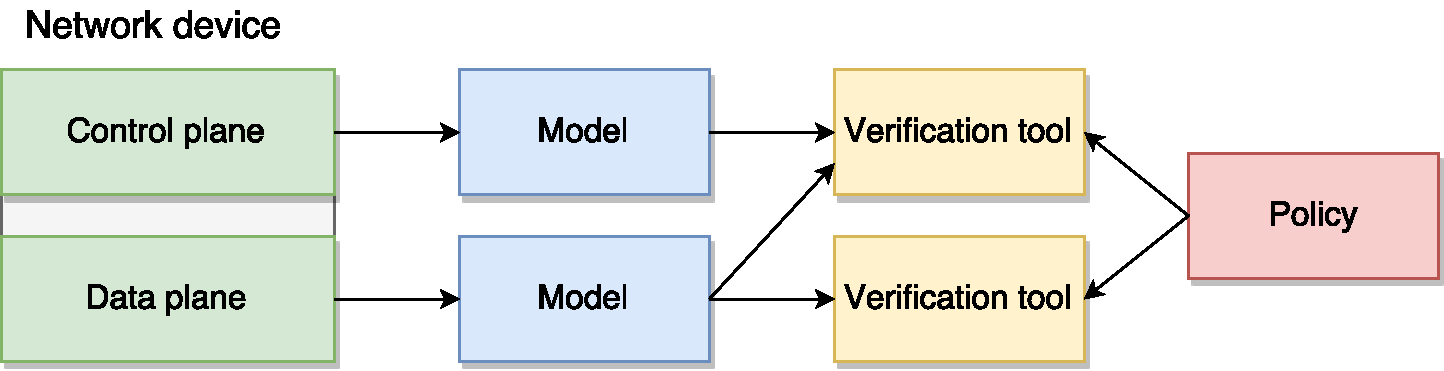
\includegraphics[scale=0.5]{src/img/control-data}
  \caption{Control/data plane verification.}
  \label{fig:control-data-verif}
\end{figure}

It is also worth briefly introducing one of the principal alternatives to
model-based static network verification, \textbf{Dynamic Network Testing} (also
known as \emph{packet injection}). As a testing technique, rather than a formal
verification one, it runs on the actual network infrastructure in a specially
configured, isolated environment.  Some network hosts, called \emph{test
agents}, generate traffic according to some test cases and evaluate the results
of each network element that is subject to testing.  However, its downsides
greatly overweight its advantages:

\begin{itemize}
  \item The search space is implicitly defined by the test cases, which means
    that a good coverage corresponds to an (exponentially) large number of
    tests.
  \item Adding to the previous point, there is an inherent bias introduced by
    having the test cases cover commonly observed behaviours, without exploring
    unexpected ones, which might lead to failures.
  \item Overall, it is more expensive to perform and requires more resources
    than static analysis.
\end{itemize}

\subsection{Static data plane verification}

Starting from the observation that including control planes in our models with
the end goal of verifying multiple properties of large (i.e.  enterprise-sized)
networks does not scale, we are left with the smaller part of each network
device: its data plane.

\begin{figure}[h]
  \centering
  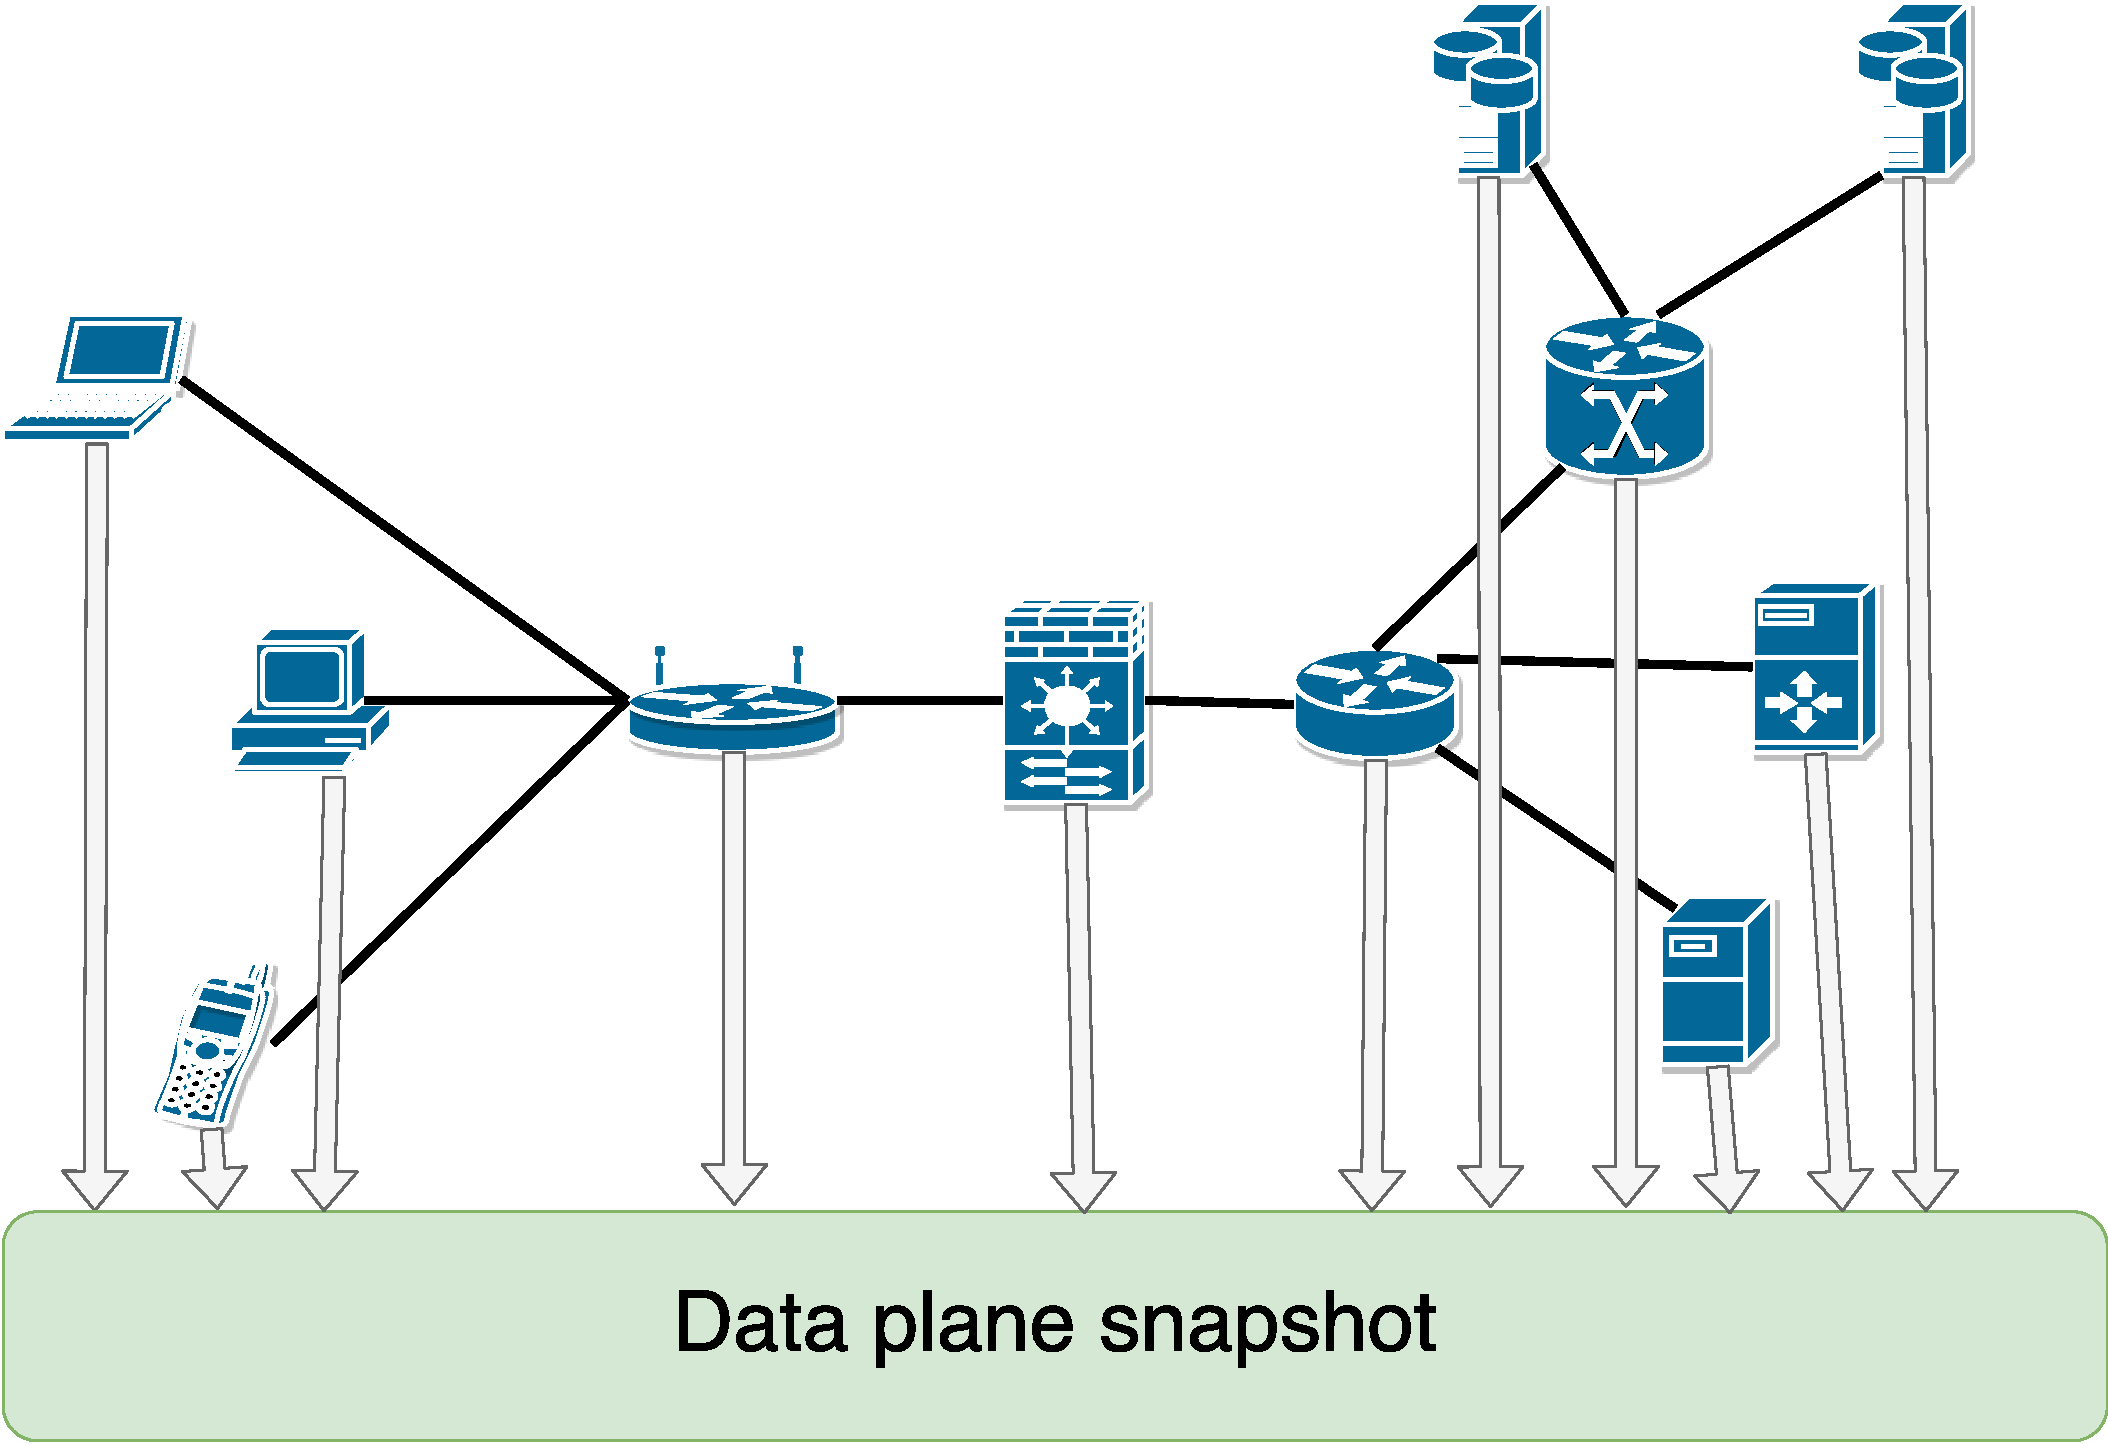
\includegraphics[scale=0.3]{src/img/data-plane-snapshot}
  \caption{Data plane/control plane decoupling.}
  \label{fig:data-plane-snapshot}
\end{figure}

Data planes (often \textbf{forwarding planes}) include only the \emph{rules}
needed by devices to expose the functionality they are designed for.  For
example, the data plane of a router is represented by its routing table, and,
possibly, packet filtering ACLs (Access Control Lists)\abbrev{ACL}{Access
Control List}.  A switch takes its decisions based on the Media Access Control
(MAC)\abbrev{MAC}{Media Access Control} table. Both of these tables are
specific instances of the more general Forwarding Information Base
(FIB)\abbrev{FIB}{Forwarding Information Base}, a name that refers to the
specialized hardware components responsible for forwarding in various network
devices.

Our limiting of the models to network data planes can be interpreted in two
opposite ways:
\begin{enumerate}[label=(\roman*)]
  \item As a downside, for ignoring the other half that makes up a network
    device: its rule-making processes, the control plane.
  \item As an approach that enables scalable verification, based on the insight
    that, even if short-lived, the data plane of a network is what dictates its
    operation at an instant.
\end{enumerate}

The second point constitutes the motivation behind the framework described in
\labelindexref{Section}{sec:symnet-sefl}.  Another way of looking at it is that
we simply ignore any process that leads to the current network
\emph{configuration} and establish whether it is a correct one or not.  If it
is, then an incremental analysis can be applied from that point forward: this
implies analyzing only the updates that reach the data plane, a technique which
has already been studied in the neighbouring field of software verification
\cite{marinescu2013katch}.  If our initial verification reports failure, human
intervention is required in order to detect the problem in the control plane
that caused the unexpected rule in the data plane.

\subsection{Symbolic execution}\label{sub-sec:symb-exec}

Symbolic execution is a means of statically analyzing a program in order to
find the inputs that cause certain parts of it to be executed.  It results in a
tree with each node representing a possible state in its execution and edges
corresponding to state transitions caused by executing the next instruction on
that specific path.  Therefore, execution paths in the analyzed program
correspond to state chains starting from the root of the symbolic execution
tree.  A state, in this context, is a collection of variables together with
their constraints expressed in terms of symbolic inputs of the program and/or
other variables.

To make things clearer, let us step through a concrete example and highlight
the construction of the symbolic execution tree
(\labelindexref{Figure}{fig:simple-tree}) for a simple C function
(\labelindexref{Listing}{lst:simple-c}):
\begin{itemize}
  \newcommand{\pa}{\hltexttt{a}}
  \newcommand{\pb}{\hltexttt{b}}
  \newcommand{\pc}{\hltexttt{c}}
  \newcommand{\vmax}{\hltexttt{max}}

  \item We assume that the \hltexttt{max3} function can be called with any
    integer numbers as arguments.  Thus, its formal parameters \pa{}, \pb{} and
    \pc{} are the input of this symbolic execution; they are assigned (pure)
    \emph{symbolic values} denoted by Greek letters $\alpha$, $\beta$ and
    $\gamma$, and together make up the initial state (i.e. the root node in the
    symbolic execution tree).  Implementation-wise, symbolic values can be
    represented as a full range of their corresponding types on the machine
    model that is targeted (e.g. $[-2.147.483.648; +2.147.483.647]$ for a
    4-bytes integer).

  \item On line 3, a new variable, \vmax{} is defined.  This is were
    language-specific behaviour comes into play, as we use the fact that the
    value of an uninitialized variable allocated on the stack is
    unspecified\footnote{From the ISO/IEC 9899:2011 standard, informally
    \textbf{C11}, paragraph \textbf{3.19.3 unspecified value} says: \emph{valid
    value of the relevant type where this International Standard imposes no
    requirements on which value is chosen in any instance}.} and we accordingly
    assign it a symbolic value.

    Note that in \labelindexref{Figure}{fig:simple-tree} variable \vmax{} is
    added to the root node due to lack of space; ideally, there should be a
    transition between the initial state (described above) and the state where
    it gets introduced.

\begin{minipage}{.45\textwidth}
\begin{listing}[H]
  \sourcecode{c}{src/code/simple-c.c}
  \caption{Simple C function used to visualize symbolic execution.}
  \label{lst:simple-c}
\end{listing}
\end{minipage}\hfill
\begin{minipage}{.45\textwidth}
\centering
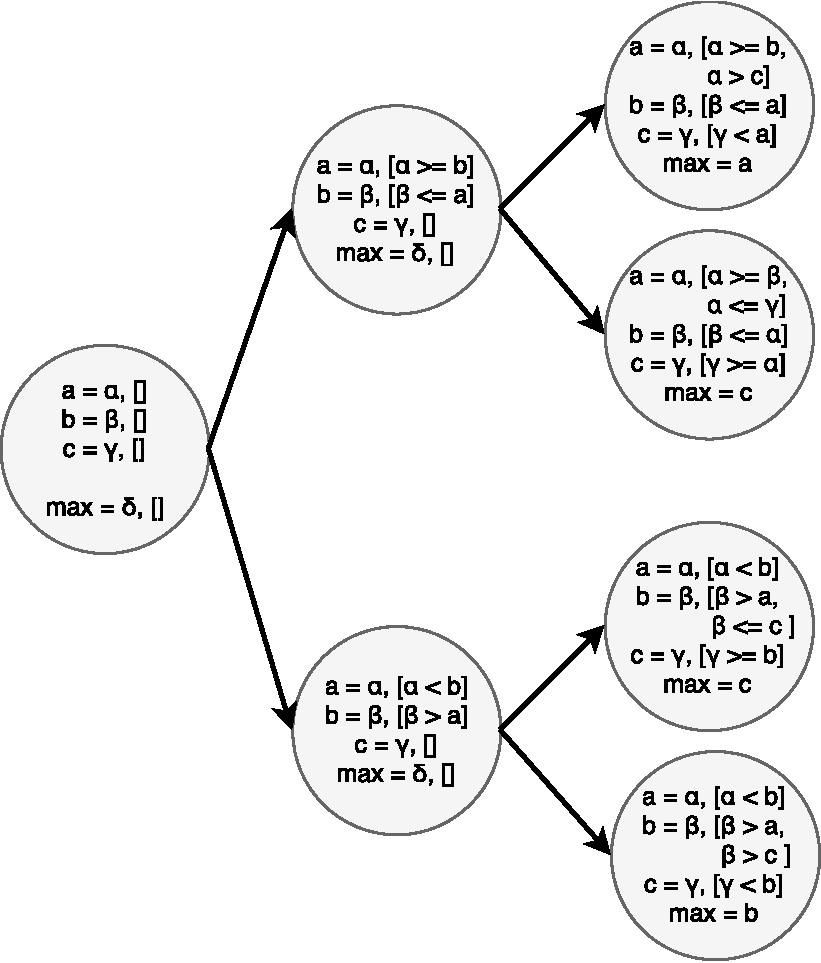
\includegraphics[scale=0.5]{src/img/symb-tree}
\captionof{figure}{Symbolic execution tree for the C function in
  \labelindexref{Listing}{lst:simple-c}.}
\label{fig:simple-tree}
\end{minipage}

  \item On line 5, the first \hltexttt{if/then/else} statement is reached,
    causing the current state to \emph{fork}, creating two child nodes that
    correspond to both scenarios: following the \hltexttt{then} part, which
    means that the condition is true, and following the \hltexttt{else} part,
    corresponding to its negation being true.  Notice that constraints are
    added to both variables \pa{} and \pb{} in each of the new states, using
    antisymmetry.

  \item Similar to the previous step, on lines 7 and 12 the inner
    \hltexttt{if/then/else} statements are symbolically executed yielding four
    more states, as well as two more constraints in each one of them.

    The interesting bit here is that variable \vmax{} loses its previously
    assigned symbolic value, $\gamma$, together with its \textbf{constraints}
    (which happens to be an empty list in this example) once it is assigned one
    of \pa{}, \pb{} or \pc{}.  It also inherits all constraints of \pa{}, which
    is not explicitly highlighted in \labelindexref{Figure}{fig:simple-tree}.
\end{itemize}

\todo{briefly what it is, an example on C code, path explosion - another
listing with many ifs}
\todo{mention KLEE, etc}

\section{SymNet and SEFL}\label{sec:symnet-sefl}

\todo{briefly present section}

\subsection{Overview}

\todo{SymNet - uses static network verification on a model of the network
constructed with a network description DSL - SEFL}
\todo{mention model - actual system equivalence issue (i.e. its usually
enforced by construction in formal verification, but we relax some constraints
(global vars, etc)}
\todo{ingress vs egress, example with if/else/if/else and switch!!}

\todo{SymNet - key novelty is SEFL, being able to model stateful networks}
\todo{SEFL - most important features, If, Constrain, :==:, :>=:, Fail, Forward}
\todo{SEFL - how we can express state}

\subsection{Building network models with SEFL}

\todo{directed graphs, nodes (commonly referred to as ports, because they also
include the actual ports of each device we model) have associated SEFL code that gets executed when
a packet reaches that node; edges - links between nodes (i.e. wires between
ports, but not only), src -> dst, many to one relation, so not really "wires".}

\subsection{Interpreting the results}

\todo{what it means to "run" SymNet - insert symbolic packet; what is symbolic
packet? etc}
\todo{what is the output - exhaustive list of possible paths together with the
constraints on each header/metadata field; hard to interpret; simplify: think
about particular rules to test and only use symbolic fields for the fields
which are of interest.}

\section{iptables}
\todo{what it is, netfilter, initial project was called netfilter/iptables;
iptables6 for IPv6 traffic, etc}

\subsection{Organization}
\todo{tables/chains, their purpose, etc}

\todo{Mention its extensions-based design and briefly discuss the two types of
extensions and give some examples.}
\paragraph{Match extensions.}
\paragraph{Target extensions.}

\subsection{Relation to Connection Tracking}
\todo{Specify that connection tracking, even if part of the netfilter project
in the kernel source code organization, is orthogonal to iptables/netfilter.
However, netfilter can look at connection tracking info to take decisions. give
example; say that another example (snat/dnat) is given below.}

\subsection{The NAT table}
\todo{Explain how NAT works, the fact that the table is analysed only when the
connection is NEW; DNAT/SNAT virtual states, --ctstate examples}
